\documentclass[russian]{lecture-notes}
\usepackage{dsfont}
\usepackage{amsmath}
\usepackage{amssymb}


\usepackage{graphicx}
\graphicspath{{pictures/}}
\DeclareMathOperator{\trk}{trk}
\DeclareMathOperator{\Krk}{Krk}
\DeclareMathOperator{\Trop}{Trop}
\DeclareMathOperator{\Brk}{Brk}
\DeclareMathOperator{\trdeg}{trdeg}

\title{Введение в тропическую математику}
\author{Дмитрий Зайков}
\date{20.07.2019}


\begin{document}
	\section{Тропическая геометрия нейронных сетей}
	
	В разделе 5 нейронные сети определяются с помощью тропической алгебры, что позволяет нам изучать их с помощью тропической алгебраической геометрии. Мы покажем, что граница принятий решений нейронной сети ~--- это подмножество тропической гиперповерхности, соответствующего тропического полинома(Раздел 6.1). Мы увидим, что в некотором смысле, зонотопы образуют геомтрические строительные блоки для нейронных сетей (Раздел 6.2). Затем мы докажем, что геометрия функции, представленной нейронной сетью, становится значиттельно более сложной с увеличением ее количества слоёв.
	\subsection{Границы решений нейронной сети}
	
	Мы будем использовать тропическую геометрию и идеи из Раздела 5 для изучения границ решений нейронных сетей, фокусируясь на случае классификации двух категорий для ясности. Как объяснено в Разделе 4, нейронная сеть $\nu : \mathbf{R}^d \rightarrow \mathbf{R}^p$ вместе с выбором функции оценки $s: \mathbf{R}^p \rightarrow \mathbf{R}$ дают нам активатор. Если выходное значение $s(\nu(x))$ превышает некоторый порог принятия решений $c$, то нейронная сеть предсказывает, что $x$ относится к одной категории (например, $x$ ~--- изображение кота), а в противном случае $x$ относится к другой категории (например, $x$ ~--- изображение собаки). Таким образом входной пространство разделено на два непересекающихся подмножества \textit{границей принятия решений $B := \{x \in \mathbf{R}^d : \nu(x) = s^{-1}(c)\} $}. Связанные области со значением выше порога и связные области со значением ниже порога будем называть \textit{положительными} и \textit{отрицательными областями} соответственно.
	
	Предоставим оценки на количество положительных и отрицательных областей и покажем, что существует тропический многочлен, чья тропическая гиперповерхность содержит границу решений.
	\begin{Proposition}
		(Тропическая геометрия границы решений). Пусть $\nu : \mathbf{R}^d \rightarrow \mathbf{R}$  ~--- $L$-слойная нейронная сеть, удовлетворяющая предположению $(a)-(c)$ с $t^{(L)} = -\infty$. Пусть функция счета $s : \mathbf{R} \rightarrow \mathbf{R}$  является иньъективной с порогом принятия решений $c$ в его диапазоне. Если $\nu = f \oslash g$, где $f$ и $g$ ~--- тропические многочлены, тогда 
		\begin{enumerate}
			\item Его граница решений $B = \{x \in \mathbf{R}^d:\nu(x) = s^{-1}(c)\}$ делит $\mathbf{R}^d$ на не более чем $N(f)$ связных положительных областей и не более, чем $N(g)$ связных отрицательных областей;
			\item Его раница решений содержится в тропической гиперповерхности тропического многочлена $s^{-1}\odot g(x)\oplus f(x) = \max\{f(x),g(x)+s^{-1}(c)\}$, то есть 
				\[B 
				\subset T(s^{-1}(c)\odot g \oplus f)
				\]  
		\end{enumerate}
	
		Функция $s^{-1}(c) \odot g \oplus f$ не обязательно линейна на каждой положительной или отрицательной области и поэтому ее тропическая гиперповерхность $T(s^{-1}(c)\odot g \oplus f)$ может дальше делить положительные или отрицательные области, полученные из $B$ на несколько линейных областей. В общем случае $\subset$ нельзя заменить на $=$.
	\end{Proposition}

	\subsection{Зонотопы, как геометрические строительные блоки нейронной сети}
	
	Из раздела 3, мы знаем, что число областей тропической гиперповерхности $T(f)$ делит пространство на равное число вершин в двойственном разбиении многоугольника Ньютона, связанного с тропическим многочленом $f$. Это позволяет нам ограничить количество линейных областей нейронной сети, ограничивая число вершин в двойственном разбиении многоугольника Ньютона. 
	
	Мы начнём изучение того, как геометрия меняется от одного слоя к следующему в нейронной сети, более точнее:
	
	\begin{Question}
		Как тропические гиперповерхности тропических многочленов в $(l + 1)$-ом слое нейронной сети связаны с ими в $l$-ом слое?
		содержимое...
	\end{Question}
	
	Рекуррентное соотношение (2) описывает, как тропические многочлены, встречающиеся в $(l + 1)$-ом слое получаются из многочленов в $l$-ом слое, а именно, через три операции: тропическая сумма, тропическую степень и тропическое умножение. Напомним, что тропическая гиперповерхность тропического многочлена ~--- двойственно разбиение многогранника Ньютона тропического многочлена, который задается проекцией верхних граней на многогранники, определяемые формулой (1). Отсюда вопрос сводится к тому, как эти три операции преобразуют многогранники, а это рассматривается в утверждениях 3.1 и 3.2. Мы следуем обозначениям из Утверждения 5.1 для следующего результата.
	
	\begin{Lemma}
		Пусть $f_i^{(l)},g_i^{(l)},h_i^{(l)}$ тропические многочлены, созданные $i$-ым узлом в $l$-ом слое нейронной сети, то есть они определяются как (2). Тогда $P(f_i^{(l)}, P(g_i^{(l)},P(h_i^{(l)}$, являющиеся подмножествами $\mathbf{R}^{d+1}$, задаются следующим образом:
		\begin{enumerate}
			\item $P(g_i^{(1) \text{ и } P(h_i^{(1)}}$ являются точками.
			\item $P(f_i^{(1)}$ ~--- отрезок.
			\item $P(g_i^{(1) \text{ и } P(h_i^{(1)}}$ ~--- зонотопы.
			\item Для $l \geq 1$,
			\[
				P(h_i^{(l)}) = Conv[P(g_i^{(l)}\odot t_i^{(l)}) \cup P(h_i^{(l)})]
			\]
			
			Если $t_i^{(l)} \in \mathbf{R}$, и $P(f_i^{(l)}) = P(h_i^{(l)})$, если $t_i^{(l)} = -\infty$
			\item Для $l \geq  1, P(g_i^{(l+1)})\text{ и } P(h_i^{(l+1)}) $ взвешены суммы Минковского, 
			\[
				P(g_i^{(l+1)}) = \sum\limits_{j=1}^{n_l} a_{ij}^-P(f_i^{(l)}) + \sum\limits_{j=1}^{n_l} a_{ij}^+P(g_i^{(l)}),
			\]
			\[
			P(h_i^{(l+1)}) = \sum\limits_{j=1}^{n_l} a_{ij}^+P(f_i^{(l)}) + \sum\limits_{j=1}^{n_l} a_{ij}^-P(g_i^{(l)})
			\]
			\[
				+\{b_ie\},
			\]
			
			Где $a_{ij}, b_i$ записаны в матрице весов $A^(l+1) \in \mathbf{Z}^{n_{l+1}\times n_l}$ и вектор смещения $b^(l+1) \in \mathbf{R}^{n_l+1} \text{ и } e:= (0, \dots,0,1)\in \mathbf{R}^{d+1}$.			
		\end{enumerate}
		\end{Lemma}
		Завершение леммы 6.2 состоит в том, что зонотопы являются строительными блоками в тропической геометрии нейронных сетей. Зонотопы широко изучены в выпуклой геометрии и, среди прочего, они тесно связаны с расположением гиперплоскостей. Лемма 6.2 связывает нейронные сети с этим обширным объёмом работы, но полный смысл этого еще предстоит изучить. В разделе С.2, кроме того, мы покажем, как можно построить эти многогранники для двуслойных нейронных сетей.
		
		\subsection{Геометрическая сложность глубоких нейронных сетей}
		
		Мы обращаемся к инструментам из раздела 3 для изучения сложности нейронной сети, показывая, что глубокая сеть более выразительна, чем неглубокая. Наша мера сложности является геометрической: мы будему следовать (Montufar et al., 2014;
		Raghu et al., 2017) и использовать количество линейных областей кусочно-линейной функции $\nu : \mathbf{R}^d \rightarrow \mathbf{R}^p$ для измерения сложности $\nu$.
		
		\begin{Theorem}
			Пусть $\nu : \mathbf{R}^d \rightarrow \mathbf{R}$ является $L$-слоем вещественной нейронной сетью с прямой связью, удовлетворяющей (a)-(c). Пусть $t^{(L)} = -\infty$ и $n_l \geq d$ для всех $l = 1,\dots,L-1$. Тогда $\nu = \nu^{(L)}$ имеет максимум
			\[
				\prod\limits_{l=1}^{L-1}\sum\limits_{i = 0}^{d} \begin{pmatrix}
				n_l\\
				i
				\end{pmatrix}
			\]
			линейных областей. В частности, если $d\leq n_1,\dots ,n_{L-1} \leq n$, то число линейных областей $\nu$ ограничено $O(n^{d(L-1)})$.
		\end{Theorem}
		
		\begin{Proof}
			Если $L = 2$, то это следует непосредственно из Леммы 6.2 и Следствия 3.4. Случай, когда $L \geq 3$ находится в разделе 7, в дополнении.
		\end{Proof}
	
	Как отмечалось в (Raghu et al., 2017), эта верхняя граница близко соответствует нижней границе $\Omega ((\frac{n}{d}^{(l-1)d})  n^d)$ в (Montufar et al., 2014, Corollary 5), когда $n_1 = \cdots = n_{L-1} = n \geq d$. отсюда мы предполагаем, что число линейных областей нейронной сети растёт полиномиально с шириной $n$ и экспоненциально с количеством слоёв $L$.
	
	\subsection{Заключение}
	
	Мы утверждаем, что прямые нейронные сети с выпрямленными узлами не что иное, как тропические рациональные карты. Чтобы понять их, нам зачастую нужно понимать соответствующую тропическую геометрию.
	
	В этой статье мы сделали первый шаг, чтобы предоставить подтверждение концепции: вопросы, касающиеся границ решений, линейных областей, как глубина влияет на выразительность и т.д. можно перевести на вопросы, касающиеся тропических гиперповерхностей, разбиений многоугольника Ньютона, многогранников, построенных из зонотопов и др.
	
	Как новая ветвь алгебраической геометрии, новшество тропической геометрии происходит из алгебры и геометрии и их взаимодействует друг с другом. Она связана множеством других областей математики. Среди прочих вещей, существует тропический аналог линейной алгебры и тропический аналог выпуклой геометрии. Мы затронули лишь небольшую часть этого богатого предмета. Мы надеемся, что дальнейшее исследование под тропическим углом поможет разгадать другие загадки глубоких нейронных сетей.
	\subsection{Дополнительный материал: Тропическая геометрия нейронных сетей}
	\begin{figure}[h]
		\center{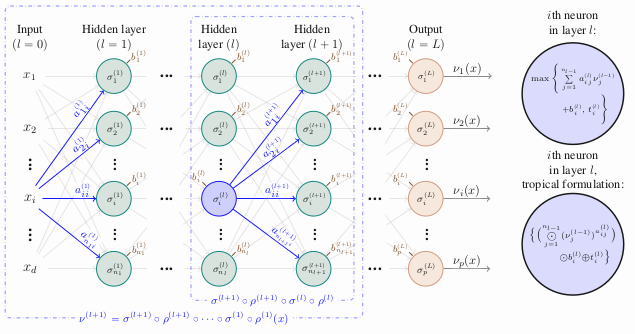
\includegraphics[scale=0.7]{1.png}}
		\caption{Общая форма ReLU прямой нейронной сети $\nu:\mathbf{R}^d \rightarrow \mathbf{R}^P$ с $L$ слоями}
	\end{figure}

	\newpage
	\subsection{Тропическая степень}
	
	В разделе 2 мы пишем $x^a = x^{\odot a}$; кроме этого небольшого злоупотребления обозначениями, $\oplus$ и $\odot$ соответствуют тропической сумме и умножению, + и - соответствуют классической сумме и умножению во всех других контекстах. Тропическая степень, очевидно, имеет следующие свойства: 
	\begin{itemize}
		\item Для $x, y \in \mathbf{R}$ и $a \in \mathbf{R}$, $a \geq 0$
		\[
			(x \oplus)^a = x^a \oplus y^a
		\]
		\[
			(x \odot y)^\alpha = x^\alpha \odot y^\alpha
		\]
		
		Если $a$ отрицательное число, то мы теряем первой свойство. В общем $(x \oplus y)^a \ne x^a \oplus y^a$ для $a < 0$. 
		\item Для $x,y \in \mathbf{R}$
		\[
			x^0 = 0
		\]
		\item Для $x \in \mathbf{R}$ и $a,b \in \mathbf{N}$
		\[
			(x^a)^b = x^{a\cdot b}
		\]
		\item Для $x \in \mathbf{R}$ и $a,b \in \mathbf{Z}$
		\[
			x^a \odot x^b = x^{a+b}
		\]
		\item Для $x \in \mathbf{R}$ и $a,b \in \mathbf{Z}$
		\[
			x^a \oplus x^b = x^a \odot(x^{a-b}\oplus 0) = x^a \odot (0\oplus x^{a-b})
		\]
	\end{itemize}
	\subsection{Примеры}
	\subsubsection{Примеры тропических кривых и двойственное разбиение многоугольника Ньютона}
	
	Пусть $f \in Pol(2,1) = \mathbf{T}[x_1,x_2]$, то есть двумерный тропический полином. В соответствии нашим рассуждениям в разделе 3 следует, что тропическая гиперповерхность $T(f)$ ~--- планарный граф двойственный двойственному разбиению $\delta (f)$ в следующем смысле:
	\begin{enumerate}
		\item  Каждой двумерной грани в $\delta (f)$ соответствует вершина в $T(f)$.
		\item Каждому одномерному ребру грани в $\delta (f)$  соответствует ребро в $T(f)$. В частности, ребро многогранника Ньютона $\Delta (f)$ соответствует неограниченному ребру в $T(f)$ , когда другие ребра соответствуют ограниченным ребрам.
		
	Рисунок 2 показывает как можно найти двойственное разбиение тропического полинома $f(x_1,x_2) = 1 \odot x_1^2\oplus 1 \odot x^2_2\oplus 2 \odot x_1x_2 \oplus 2 \odot x_1 \oplus 2 \odot x_2 \oplus 2$. Во-первых, найдем выпуклую оболочку 
	\[
		P(f) = Conv\{(2,0,1),(0,2,1),(1,1,2),(1,0,2),(0,1,2),(0,0,2)\}
	\]
	Тогда, проецируя верхнюю оболочку $P(f)$ на $\mathbf{R}^2$, мы получим $\delta(f)$, двойственное разбиение многоугольника Ньютона.
	\end{enumerate}
	\subsubsection{Многогранники двухслойной нейронной сети }
	Продемонстрируем наши рассуждения в Разделе 6.2 на двухслойном примере. Пусть $\nu :\mathbf{R}^2 \rightarrow \mathbf{R}$ будет с $n_0=2$ входными узлами, $n_1 = 5$ в первом слое и $n_2 = 1$ узлов в выходе:
	\[
		y = \nu^{(1)}(x) = \max 
		\begin{Bmatrix}
			\begin{bmatrix}
			-1 &1 \\
			1 &-3 \\
			1 &2 \\
			-4 &1\\
			3 &2 
			\end{bmatrix}
		\begin{bmatrix}
		x_1\\
		x_2
		\end{bmatrix} 
		+ \begin{bmatrix}
		1\\
		-1\\
		2\\
		0\\
		-2
		\end{bmatrix}, 0
		\end{Bmatrix}
	\]
	\[
		y = \nu^{(2)}(y) = \max\{y_1 + 2y_2 + y_3 - y_4 - 3y_5, 0\}
	\]
	
	Сначала мы выражаем $\nu^{(1)}$ и $\nu^{(2)}$, как тропическое рациональное отображение.
	\[
	\nu^{(1)}=F^{(1)}\oslash G^{(1)} , \nu^{(2)} \oslash g^{(2)},
	\]
	Где 
	\[
		y:=F^{(1)}(x) = H^{(1)}(x) \oplus G^{(1)}(x)
	\]
	\[
		z:=G^{(1)}(x) = \begin{bmatrix}
		x_1\\
		x_2^3\\
		0\\
		x_1^4\\
		0
		\end{bmatrix}
	\]
	\[
		H^{(1)}(x) = \begin{bmatrix}
		1\odot x_2\\
		(-1)\odot x_1\\
		2 \odot x_1x^2_2\\
		x_2\\
		(-2)\odot x_1^3 x^2_2
		\end{bmatrix}
	\]
	и 
	\[
		f^{(2)}(x) = g^{(2)}(x) \oplus h^{(2)}(x)
	\]
	\[
		g^{(2)}(x) = y_4 \odot y_5^3 \odot z_1 \odot z_2^2 \odot z_3 = (x_2 \oplus x^4_1) \odot ((-2)\odot x^3_1x^2_2 \oplus 0)^3 \odot x_1 \odot (x_2^3)^2
	\]
	\[
		h^{(2)}(x) = y_1 \odot y_2^2 \odot y_3 \odot z_4 \odot z_5^3 = (1 \odot x_2 \oplus x_1)\odot ((-1)\odot x_1 \oplus x^3_2)^2 \odot (2 \odot x_1x_2^2 \oplus 0) \odot x_1^4.
	\]
	\begin{figure}[h]
		\center{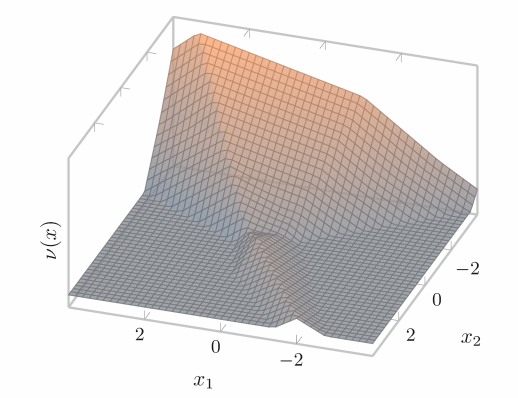
\includegraphics[scale=0.5]{2.png}}
	
	\end{figure}
	Запишем $F^{(1)} = (f_1^{(1)}, \dots, f_5^{(1)})$ и аналогично для $G^{(1)}$ и $H^{(1)}$. Мономы встречающиеся в $g_j^{(1)}(x)$ и $h_j^{1)}(x)$ являются всеми формами $cx_1^{\alpha_1}x_2^{\alpha_2}$. Следовательно $P(g_j^{(1)})$ и $P(h_j^{(1)})$ ~--- точки в $\mathbf{R}^3$
	
	Так как $F^{(1)} = G^{(1)} \oplus H^{(1)} ,P(f_j^{(1)})$ ~--- выпуклая оболочка двух точек, и является отрезком в $\mathbf{R}^3$. Многоугольники Ньютона связаны с $f_j^{(1)}$, равные их двойственным разбиениям, в этом случае, полученные проецированием этих отрезков на плоскость, натянутую на $\alpha_1, \alpha_2$, что показано на рисунке ниже.
	
	В всех рисунках ниже, двойственные разбиения были проведены вдоль направления $c$(вниз) и отделены от многогранников для наглядности.
	\begin{figure}[!h]
		\center{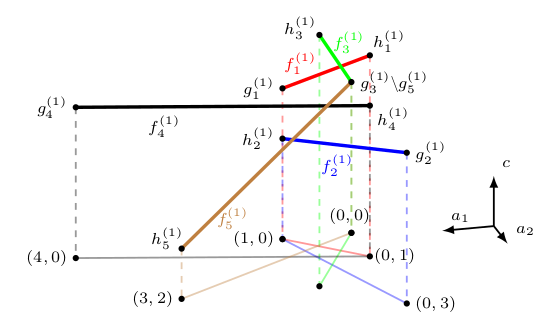
\includegraphics[scale=0.7]{3.png}}
		\caption{$P(F^{(1)})$ и двойственное разбиение $F^{(1)}$}
		
	\end{figure}
\newpage
	\begin{figure}[!ht]
		\center{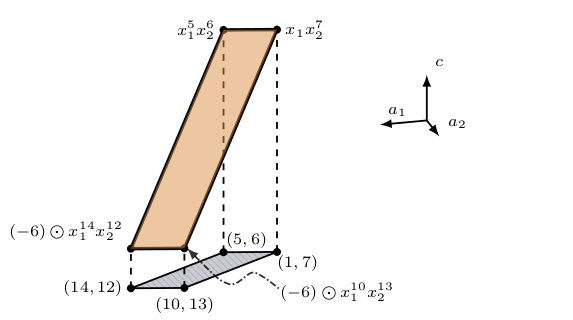
\includegraphics{4.png}}
		\caption{$P(g^{(2)})$ и двойственное разбиение $g^{(2)}$}
	\end{figure}

\newpage
	\begin{figure}[!ht]
		\center{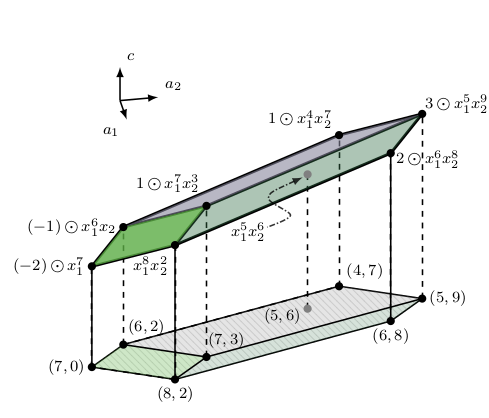
\includegraphics{5.png}}
		\caption{Многогранник, связанный с $h^{(2)}$ и его двойственное разбиение}
		
	\end{figure}
	\newpage
	\begin{figure}[!ht]
		\center{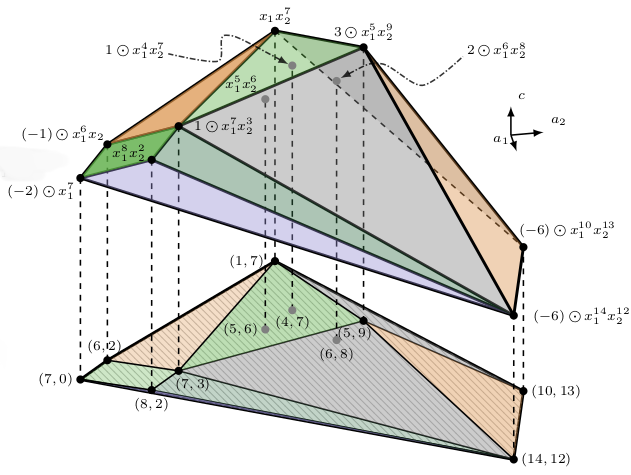
\includegraphics{6.png}}
		\caption{$P(f^{(2)})$ и двойственное разбиение $f^{(2)}$}
	\end{figure}
	
	\newpage
	\newpage
	Отрезки $P(f_j^{(1)}), j =1,\dots,5$ и точки $P(g_j^{(1)})j =1,\dots,5$,служат в качестве строительных блоков для $P(h^{(2)})$ и $P(g^{(2)})$, которые простроенны, как взвешенные суммы Минковского:
	\[
		P(h^{(2)}) = P(f^{(1)}_4) +  3P(f^{(1)}_5) +  P(g^{(1)}_1) + 2P(g^{(1)}_2) + P(g^{(1)}_3)
	\]
	\[
		P(g^{(2)}) = P(f^{(1)}_1) +  2P(f^{(1)}_2) +  P(f^{(1)}_3) + P(g^{(1)}_4) + 3P(g^{(1)}_5)
	\]
	
	
	

\end{document}